\documentclass{article}

% if you need to pass options to natbib, use, e.g.:
%     \PassOptionsToPackage{numbers, compress}{natbib}
% before loading neurips_2020

% ready for submission
% \usepackage{neurips_2020}

% to compile a preprint version, e.g., for submission to arXiv, add add the
% [preprint] option:
    \usepackage[final, nonatbib]{mlres2022}

% to compile a camera-ready version, add the [final] option, e.g.:
%     \usepackage[final]{neurips_2020}

% to avoid loading the natbib package, add option nonatbib:
 %    \usepackage[nonatbib]{neurips_2020}

\usepackage[utf8]{inputenc} % allow utf-8 input
\usepackage[T1]{fontenc}    % use 8-bit T1 fonts
\usepackage{url}            % simple URL typesetting
\usepackage{booktabs}       % professional-quality tables
\usepackage{amsfonts}       % blackboard math symbols
\usepackage{nicefrac}       % compact symbols for 1/2, etc.
\usepackage{microtype}      % microtypography
\usepackage{graphicx}
\usepackage{amsmath}
\usepackage{algorithm}
\usepackage{algorithmic}
\usepackage{subcaption}
\usepackage{multirow}
\usepackage{hyperref}       % hyperlinks
\usepackage[ 
	backend=bibtex8,     
    style=authoryear,	
    maxcitenames=2,      
    maxbibnames=25,  
    dashed = false,		
    hyperref=true,       
    bibencoding=inputenc,   
    useeditor=false,  
    uniquename=init,  
    doi=true,
    url=false,
    isbn = false,
    giveninits = true,
    natbib=true
]{biblatex}
	
\addbibresource{literature.bib}

\title{Denoising Forecasts: Leveraging Diffusion Models for Predicting Renewable Energy Supply}

% The \author macro works with any number of authors. There are two commands
% used to separate the names and addresses of multiple authors: \And and \AND.
%
% Using \And between authors leaves it to LaTeX to determine where to break the
% lines. Using \AND forces a line break at that point. So, if LaTeX puts 3 of 4
% authors names on the first line, and the last on the second line, try using
% \AND instead of \And before the third author name.

\author{Swadesh Jana \\
Student ID: 6661704 \\
Master Machine Learning}

\begin{document}

\maketitle

\begin{abstract}
Weather-dependent energy output forecasting systems have suffered due to the inherent noise in weather elements. Diffusion models can improve such forecasting by learning these noise patterns. In this work, we show that diffusion models can be used on top of any regression-based model for better forecasting. The quality of forecasting is improved by the denoising
diffusion-based conditional generative model over a pre-trained conditional mean
estimator. The conditioning prior model and the diffusion model are trained and tested using the RMSE metric on a dataset containing 4 years of hourly weather data with corresponding solar and wind energy supply values. It is observed that the diffusion mechanism consistently outperforms the initial conditioning prior by 4-5\% on average. On the solar 1-hour forecast, the diffusion model improves the RMSE from 86.11 to 81.4 while for the corresponding wind data, it improves from 188.57 to 178.35. By carefully tuning the hyperparameters, it is possible to obtain higher improvements as well without much bells-and-whistles. The code is available at \url{https://github.com/Swadesh13/Renewable-CARD}.
\end{abstract}

\section{Introduction}

In the realm of renewable energy supply forecasting, accurate predictions are important for efficient grid management and resource allocation. However, traditional forecasting models often grapple with inherent noise and uncertainty, leading to less reliable predictions due to the variability and intermittency of natural phenomena.

A diverse array of methods for renewable energy supply forecasting have been successfully published as outlined in Section \ref{sec:related-works}. However, most of these methods suffer from being unable to utilize either the underlying noisy variations in the data or the temporal information effectively. A compelling alternative arising recently are diffusion models. Diffusion models have become increasingly popular following their success in generative tasks, particularly image synthesis \citep{dhariwal2021diffusion,ramesh2022hierarchical}. %These models excel in generating high-quality, diverse samples by iteratively refining random noise into coherent outputs, guided through learned probabilistic distributions. 
The models effectively manage and propagate uncertainties through stochastic differential equations, capturing the random evolution of variables over time, thus generating high-quality, diverse samples. In this work, the following contributions have been made:
\begin{enumerate}
  \item Diffusion-based regression models have been used for forecasting the solar and wind energy supplies in Germany. Given the weather data at any timestep, the models predict the energy output in a 1-hour and a 24-hour interval. %This is made possible through injecting covariate dependence and a pre-trained conditional mean estimator into both the forward and reverse diffusion chains.
  \item Due to the probabilistic output of the models, they are evaluated based on the root-mean-square error (RMSE) along with graphs that help to provide a clear discussion of the results.
  \item Various neural network architectures along with hyperparameter tuning have been performed to find the most suitable model for the forecasting task.
\end{enumerate}

In the following sections, the related works, methodology used for the modeling, the training strategies and the results have been discussed.

\section{Related Works} \label{sec:related-works}

A number of models including statistical time series analysis \citep{9209858}, machine learning models, artificial neural networks, particularly feedforward and recurrent neural networks \citep{hossain2020short, lim2022solar}, and also physical simulation models have been used for solar and wind power forecasting. A comprehensive study has been provided by \citet{tawn2022review}. Diffusion methods have been extensively discussed in Section \ref{sec:method}. Although there has not been a comprehensive study on diffusion models in renewable power supply forecasting, \citet{hatanaka2023diffusion} discusses solar forecasting using diffusion models. The implementation of diffusion models for this paper has been derived from the CARD models \citep{han2022card}.

\section{Methodology} \label{sec:method}

Forecasting of solar and wind energy outputs at any point of time can be considered a regression task where the inputs are weather conditions on a temporal domain and the output is the energy output or, in this case, a probabilistic distribution of the possible values. In this section, the general diffusion process along with its implementation in a regression problem have been discussed.

\subsection{Diffusion process}

A forward diffusion process \citep{sohl2015deep} starts at some starting point $y_0 \sim q$, where $q$ is the probability distribution to be learned. Then, it repeatedly adds noise to $y_{t-1}$ by 
\begin{equation} \label{eqn:diff_noise}
  y_t = \sqrt{1-\beta_t} y_{t-1} + \sqrt{\beta_t}\epsilon_t,
\end{equation}
where $\beta_1,\dots,\beta_T \in (0, 1)$ are fixed constants, and $(\epsilon_1,\dots,\epsilon_T)$ are IID samples from $\mathcal{N}(0, I)$. 
% This makes sure that for any starting $y_0$, we have $\lim_t y_t|y_0$ converges to $\mathcal{N}(0, I)$. 
% Thus, at any time $t$,
% \begin{equation}
%   q(y_t;y_{t-1}) = \mathcal{N}(y_t ; \sqrt{\alpha_t}y_{t-1}, \beta_tI),
% \end{equation}
% where $\alpha_t = 1 - \beta_t$. However, 
Following \citet{han2022card}, a prior knowledge of the relation between the original feature vector $x$ and $y_0$ learned by a neural network (NN), $f_\phi(x)$ is also added. 
Thus, the forward process can be written as:
\begin{equation}
  q(y_t | y_{t-1}, f_\phi(x)) = \mathcal{N}(y_t ; \sqrt{\alpha_t}y_{t-1} + (1-\sqrt{\alpha_t})f_\phi(x), \beta_tI),
\end{equation}
where $\alpha_t = 1 - \beta_t$.

The forward process is a product over multiple timesteps and thus, also a normal distribution: $\mathcal{N}(y_t; \sqrt{\bar{\alpha}_t}y_0 + (1-\sqrt{\bar{\alpha}_t})f_\phi(x), (1-\bar{\alpha}_t)I)$, where $\bar{\alpha}_t = \prod_t\alpha_t$.

% The entire forward diffusion process becomes,
% \begin{equation}
%   q(y_t|y_0,x) = q(y_t|y_0,f_\phi(x)) = \mathcal{N}(y_t; \sqrt{\bar{\alpha}_t}y_0 + (1-\sqrt{\bar{\alpha}_t})f_\phi(x), (1-\bar{\alpha}_t)I),
% \end{equation}
% where $\bar{\alpha}_t = \prod_t\alpha_t$.


% The entire diffusion process can be written as,
% \begin{equation}
%   q(y_{0:T}) = q(y_0)q(y_1|y_0)\cdots q(y_T|y_{T-1}) = q(y_0)\mathcal{N}(y_1;\sqrt{\alpha_t}y_0,\beta_1 I) \cdots \mathcal{N}(y_T;\sqrt{\alpha_T}y_{T-1},\beta_T I)
% \end{equation}
%% or,
%% \begin{equation}
%%   \ln q(x_{0:T}) = \ln q(x_0) - \sum_{t=1}^T \frac{1}{2\beta_t} ||x_t-\sqrt{\alpha_t}x_{t-1}||^2 + C,
%% \end{equation}
%% where $C$ is a normalization constant and can be omitted.
From here, we can derive through standard manipulation of Gaussian process, that 
% \begin{equation}
%   y_t|y_0 \sim \mathcal{N}(\sqrt{\bar{\alpha}}y_0, (1-\bar{\alpha_t})I),
% \end{equation}
% and
\begin{equation}
  q(y_{t-1}|y_t,y_0,f_\phi(x)) = \mathcal{N}(y_{t-1}; \tilde{\mu}_t(y_t, y_0, f_\phi(x)), \tilde{\beta_t}I),
\end{equation}
where 
\begin{align*}
  &\tilde{\mu}_t = \frac{(1-\bar{\alpha}_{t-1})\sqrt{\alpha_t}}{1-\bar{\alpha}_t}y_t + \frac{\beta_t\sqrt{\bar{\alpha}_{t-1}}}{1-\bar{\alpha}_t}y_0 + \biggl(1 + \frac{(\sqrt{\bar{\alpha}_t}-1)(\sqrt{\alpha_t}+\sqrt{\bar{\alpha}_{t-1}})}{1-\bar{\alpha}_t}\biggl)f_\phi(x), \\
  &\tilde{\beta_t} = \frac{1-\tilde{\alpha}_{t-1}}{1-\tilde{\alpha}_{t}}\beta_t.
\end{align*}

\begin{figure}[ht]
  \centering
  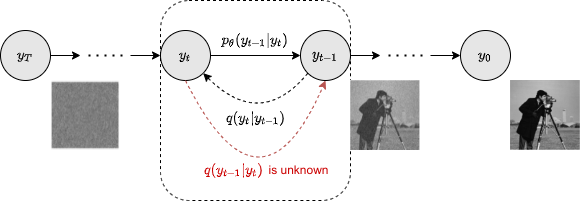
\includegraphics[width=0.75\textwidth]{diffusion.png}
  \caption{The diffusion process visualization with the example of denoising an image. $y_T$ is the initial noise, $p_\theta$ is the trained posterior that tries to learn the noise to be removed from the image at some time step $y_t$. The forward Gaussian process is represented by the successive $q(y_t|y_{t-1})$.}
  \label{fig:diffusion}
\end{figure}


Using the denoising diffusion probabilistic models (DDPM) method \citep{ho2020denoising}, the reverse diffusion process is characterized as the joint distribution $p_\theta(y_{0:T})$ with learnable parameters $\theta$, and is a Markov chain with learned Gaussian transitions starting at $p(y_T|x) = \mathcal{N}(y_T;f_\phi(x),I)$. This is shown in Fig. \ref{fig:diffusion}. %:
% \begin{align}\label{eqn:p_theta}
%   & p_\theta(y_{0:T}|x) = p(y_T|x)\prod_{t=1}^{T}p_\theta(y_{t-1}|y_t, x), \text{where} \\ & p_\theta(y_{t-1}|y_t,x) = \mathcal{N}(y_{t-1}; \mu_\theta(y_t, x, t), \Sigma_\theta(y_t, x, t))
% \end{align}
Therefore, the goal is to learn the parameters such that $p_\theta(y_{t-1}|y_t,x)$ is as close to $q(y_{t-1}|y_t,y_0,f_\phi(x))$ as possible. This is possible through variational inference, i.e. performing the negative log likelihood (NLL) and using the Evidence Lower Bound (ELBO) inequality:
% \begin{equation}
%   \mathbb{E}_{y_0\sim q}[-\log p_\theta(y_0|y_1,x)] \le \mathbb{E}_{y_{0:T}\sim q}\left[-\log \frac{p_\theta(y_{0:T}|x)}{q(y_{1:T}|y_0,f_\phi(x))} \right] = L(\theta),
% \end{equation}
% which can be simplified to
\begin{equation}
  L(\theta) = \sum_{t=1}^T \mathbb{E}_{y_{t-1},y_t\sim q}\left[-\ln p_\theta(y_{t-1}|y_t,x) \right] + \mathbb{E}_{y_0\sim q}\left[ D_{KL}(q(y_T | y_0, f_\phi(x)) || p_\theta (y_T | x)) \right] + C,
\end{equation}
where $L(\theta)$ is the loss function of the whole process, $D_{KL}$ is the Kullback-Leibler Divergence, and $C$ is a constant term. Since $p_\theta(y_T|x)$ is a normal distribution that does not depend on $\theta$, we can ignore the last two terms and write the loss function as a sum of steps:
\begin{equation}\label{eqn:loss_final}
  L(\theta) = \sum_{t=1}^T L_t\ \text{with}\ L_t(x, y_t, f_\phi(x), t) = \mathbb{E}_{y_{t-1},y_t\sim q} \left[-\ln p_\theta(y_{t-1}|y_t,x) \right]
\end{equation}

% The $L_t$ is now used for optimization of the parameters $\theta$ that has been described in the following section.

\subsection{Regression using Diffusion}

The general diffusion process can be regarded as a probabilistic regression process to gradually recover the distribution of the noise term, the aleatoric or local uncertainty inherent in the observations \citep{kendall2017uncertainties}. Here, in addition to the original process, the learned prior $f_\phi$ is also used. In Eq. \ref{eqn:loss_final}, the main term is $p_\theta$ which has mean $\mu_\theta$ and variance $\Sigma_\theta$. Using the method from \citet{ho2020denoising}, $\Sigma_\theta$ is set to $\sigma_t^2I$, where $\sigma_t^2=\tilde{\beta}_t$. $y_t$ can be written as 
% \begin{equation}
  $y_t = \sqrt{\bar{\alpha}_t}y_0 + \sqrt{1-\bar{\alpha}_t}\epsilon + (1-\sqrt{\bar{\alpha}_t})f_\phi(x)$
% \end{equation}
from eq. \ref{eqn:diff_noise} to which $f_\phi(x)$ is also added. A reparameterization of the equations leads to $\mu_\theta$ being computed as 
\begin{equation}
  \mu_\theta = \frac{1}{\sqrt{\alpha_t}}\biggl(y_t-(1-\sqrt{\bar{\alpha}_t})f_\phi(x)-\sqrt{1-\bar{\alpha}_t}\epsilon_\theta(x,y_t,f_\phi(x),t)\biggr),
\end{equation}
where $\epsilon_\theta$ is a function approximator intended to predict $\epsilon$. Thus, it can be a function of any parameters that are already known at any given timestamp $t$, as written above. Now, the aim is to optimize $\epsilon_\theta$.

The algorithm for the training and inference process have been expressed in \ref{alg:reg_form_1_train} and \ref{alg:reg_form_1_inf} respectively. For training, the model (i.e. the parameters $\theta$) learns the noise at any random timestep $t \in [0, \dots, T]$, while during inference, the model is repeatedly passed through $T$ steps to get the predicted output, which for a diffusion model will be a distribution. 

In Alg. \ref{alg:reg_form_1_inf}, $\hat{ y}_0$ is the reparameterized $\mu_\theta$ value for $t=0$. It is important to note that the inference algorithm is repeated multiple times (parallelly) to get a mean forecast. This helps to obtain a mean forecast independent of the initial noise. As will be seen further, for certain tasks, taking certain percentiles of the distribution is better than just the mean or median.

\noindent\begin{minipage}{0.47\textwidth}
\begin{algorithm}[H]
  \begin{algorithmic}[1]
    \STATE Pre-train $f_{\phi}(x)$ that predicts $\mathbb{E}(y | x)$
    \REPEAT
    \STATE Draw $y_0\sim q( y_0 | x)$
    \STATE Draw $t\sim \text{Uniform}(\{1\dots T\})$
    \STATE Draw $\epsilon\sim\mathcal{N}(0, I)$
    \STATE Perform numerical optimization on\\ $\nabla_\theta \big|\big|\epsilon - \epsilon_\theta\big(x, y_t, f_{\phi}( x), t\big)\big|\big|^2$
    \vspace*{4pt}
    \UNTIL Convergence
  \end{algorithmic}
  \caption{Training}
  \label{alg:reg_form_1_train}
\end{algorithm}
\end{minipage}
\hfill
\noindent\begin{minipage}{0.49\textwidth}
\begin{algorithm}[H]
  \begin{algorithmic}[1]
    \STATE $ y_T\sim\mathcal{N}(f_{\phi}( x), I)$
    \FOR{$t=T$ to $1$}
    \STATE Draw $ z\sim\mathcal{N}(0, I) $ if $t>1$
    \STATE Calculate reparameterized $\hat{ y}_0$
    \STATE Let $ y_{t-1}=\gamma_0\hat{ y}_0+\gamma_1 y_t+\gamma_2f_{\phi}( x)+\sqrt{\tilde{\beta}_t} z$ \\ if $t>1$, else set $ y_{t-1}=\hat{ y}_0$
    \ENDFOR
    \STATE \textbf{return} $ y_0$
  \end{algorithmic}
  \caption{Inference}
  \label{alg:reg_form_1_inf}
\end{algorithm}
\end{minipage}  

\subsection{Choosing prior and guidance models}

As stated above, there are two parameters that have been introduced, viz. $\phi$ (or $f_\phi$) and $\theta$ (or $\epsilon_\theta$). The diffusion process can be considered as a secondary step over the predictions of $\phi$ on input features. Thus, $\phi$ is a regular neural network (NN) model that solves a regression model. In this paper, the NN model considered is a LSTM block followed by a simple feedforward linear neural network with activations. Theoretically, it can be any regression model.

On the other hand, $\theta$ is a guidance model that tries to learn the noise in the diffusion process. Its architecture has been derived from \citet{han2022card}. The inputs $x, y_t,f_\phi(x)$ are concatenated and sent through three fully-connected layers. Hadamard product between each of the output vector with the corresponding timestep embedding is computed, followed by a softplus non-linearity. Lastly, we apply a fully-connected layer maps the vector to the output forward diffusion noise prediction.


\section{Evaluation}

In this section, the dataset, input and output data formats, training strategies and the evaluation metrics have been discussed.

\begin{figure}[t]
  \centering
  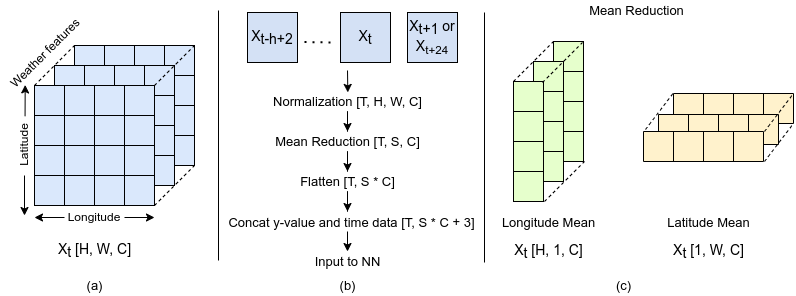
\includegraphics[width=1\textwidth]{data-proc.png}
  \caption{(a) A data matrix at any point in time, (b) T=h time frames are used including the future time step and processed as shown, (c) the two mean reduction methods viz., latitude and longitude used for the study. Note: $[\cdot]$ represents the shape of the data after applying the transformation and $S$ is the resultant shape ($H*1$ or $1*W$) after the respective reductions. In general, H=8, W=10, C=8. Additionally, here $T$ denotes the previous time steps of the data and not the diffusion process and $t$ refers to the data point at a particular time t.}
  \label{fig:data-proc}
\end{figure}

\subsection{Dataset}

The dataset provided is the German weather dataset for 4 years (2019-2022) with hourly intervals. It is arranged in the form of a 3-dimensional matrix, where two dimensions are the latitudes (8) and longitudes (10), while the third is the feature axis. Alongside it, is the photovoltaic and the wind power output (cumulated over Germany) dataset with 15-minute intervals for the same time period. The 15-minute power outputs are averaged in groups of 4 to get 1-hour intervals. Since all columns are not relevant for wind and solar energy outputs, they are divided according to the power type. For wind energy, the features are geopotential (column name: z), mean sea level pressure (msl), u10, v10, u100, v100, temperature 2m above ground (t2m), and boundary layer height (blh), where u denotes the u-component of the wind speed, v is the v-component, and the numbers are the altitude at which the wind speed is measured. For solar energy, clear-sky direct solar radiation at surface (cdir), total cloud cover (tcc), t2m, surface net solar radiation (ssr), top net solar radiation (tsr), sunshine duration (ssd), forecast surface roughness (fsr) and total precipitation (tp) are used. A few additional pre-processing are also applied as follows: 
\begin{enumerate}
  \item Certain features such as ssr, tsr, fsr, ssd, tp are cumulated over the day. But it will be more useful for the model to get the values over the last hour. Therefore, they are subtracted from the previous hour value to get the density.
  \item Past power output data is also made available to the model. This makes it easier to understand the range over which the future output is possible.
  \item Feature scaling using mean and square root of variance to get normalized feature values.
  \item Add time in the form of hours of the day, and the month of the year after passing them through a sin function to retain the periodicity.
  \item The data in the original form is a 4 dimensional matrix, which when reduced to 1 dimensional vector has a dimension of $7*8*10*8=4480$. Thus, longitude and latitude mean reduction steps are employed, where for each feature the values are averaged over the longitude or the latitude axes respectively, as shown in Fig. \ref{fig:data-proc}(c). 
\end{enumerate}

The data processing steps are shown in Fig. \ref{fig:data-proc}. There are two forecasts to be made: 1-hour and 24-hour ahead. Let there be a window of $h$ hours in the past that is used for the forecast at time $t$. Therefore, the input data is $[X_{t-h+1}, \dots, X_{t}]$ where $X$ denotes the respective features at that timestamp, to predict either the $y_{t+1}$ or $y_{t+24}$ energy outputs.  

\subsection{Training Strategy}

The models are trained on four different datasets: solar with 1-hour (S-1) and 24-hour (S-24) forecast and wind with the same forecast (W-1 \& W-24). The deterministic NN is first pre-trained on the datasets for 1000 epochs and then the guidance probabilistic NN is trained for 1000 epochs, always with a batch size of 256. The optimizer is Adam with initial learning rate of $10^{-3}$ and further stepped down by a factor of 0.1 every 400 epochs. It is observed that gradient clipping of 1 (L2 norm) helps to stabilize the training process. The loss functions used are L1 for wind prior conditioning, L2 for all other training processes. 

After some hyperparameter tuning, it is observed that the best window sizes are 7 for S-1, 13 for S-24, 5 for W-1 and 7 for W-24. It is also observed that appending the original data to the prior conditioning prediction helps in the wind forecast but does not help for the solar forecasts. As shown later, the solar energy outputs have a simple distribution over time and thus, might not need a lot of data for accurate predictions.

The Root Mean Square Error (RMSE) evaluation metric has been computed on the 2022 test data both on the predicted distribution of the data and the mean of the distribution. It measures the square root of the L2 loss between the forecasted energy value and the true value. Mathematically, over N samples, it can be written as:
\begin{equation}
  RMSE(y, \hat{y}) = \biggl(\frac{1}{N}\sum_{i=1}^{N}(\hat{y}_i - y_i)^2\biggl)^{\frac{1}{2}},
\end{equation}
where $\hat{y}_i$ is the $i$-th forecasted value and $y_i$ is the corresponding true value.

\section{Results \& Discussion}

\begin{table}[h]
  \centering
  \setlength{\tabcolsep}{10pt}
  \begin{tabular}{lllllllllllll}
    \toprule
    Model & Solar-1 & Solar-24 & Wind-1 & Wind-24\\
      \midrule
    NN-Lat & 86.11 & 481.22 &  190.74 & 986.11 \\
    NN-Lat-Diff & \textbf{81.4} ! (5.8\%) & \textbf{333.72} ! (30.7\%) & 180.95 (5.1\%) & 931.21 (2.3\%) \\
    NN-Lon & 95.28 & 505.31 &  188.57 & 953.06 \\
    NN-Lon-Diff & 90.75 ! (4.8\%) & 390.21 ! (23\%) & \textbf{178.35} (5.3\%) & \textbf{963.43} (2.3\%) \\
    \bottomrule
    \vspace*{0.2cm}
  \end{tabular}
  \caption{Results for each dataset type. Diff means diffusion aided model. Lat means longitude reduction and thus latitude information is still kept, while Lon is vice versa. (\%) refers to the improvement over the NN model. Note: ! - means the 70-th (S-1) and the 100-th (S-24) percentiles are taken instead of the mean over the predicted forecasts.}
  \label{tab:results}
\end{table}

The results for each data type are provided in Table \ref{tab:results}. Diffusion process consistently improves on the RMSE scores obtained by the original conditioning LSTM-based NN model. Longitude reduction of the data aids the solar energy output forecasting while latitude reduction can be found to be better for wind energy forecasting.

For wind energy forecasting, the model is able to accurately predict the energy output patterns for the 1-hour forecast as shown in Fig. \ref{fig:wind-1-diff}. The accuracy decreases for the 24-hour forecast (Fig. \ref{fig:wind-24}), but is still able to predict the average pattern except the sharp fluctuations that might be due to other external reasons as well. The corresponding values in Table \ref{tab:results} show that the best possible RMSE obtained are 178.35 and 963.43 respectively for the W-1 and W-24 forecasts.

The solar energy output forecasting, on the other hand, requires some more analysis before making final conclusions. As seen in Fig. \ref{fig:solar-1} and \ref{fig:solar-1-zoom}, the true solar values form a periodic Gaussian-like shape, that is much easier to predict. However, the forecasts seem to mostly miss the peaks. Fig. \ref{fig:solar-1-zoom-diff} shows how the overall diffusion forecast distribution is able to cover the maxima for each day. Thus, by taking a higher percentile of all the predictions at each point of time, it is possible to increase the scores. As seen in Table \ref{tab:results}, the RMSE for S-1 and S-24 are 81.4 (70-th percentile) and 333.72 (100-th percentile) respectively. For the 24-hour forecasts, as observed in Fig. \ref{fig:solar-24}, even the 100-th percentile (the highest point of the distribution), is well below the true energy output peaks. The difference is found to be maximum for the higher peaks. This can be attributed to the fact that the model has no information on the last 24 hours energy outputs.


\begin{figure}[t]
  \centering
  \begin{subfigure}{.45\textwidth}
    \centering
    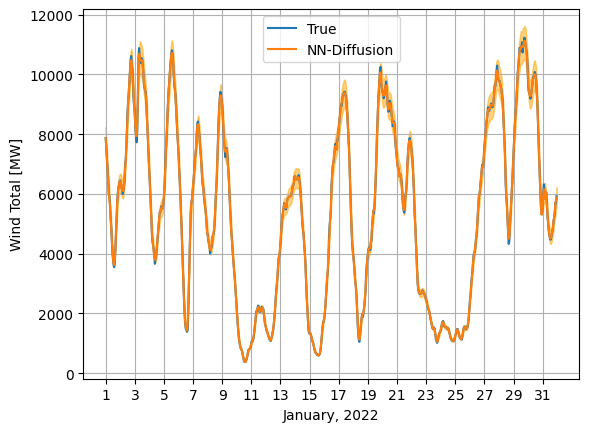
\includegraphics[width=1\linewidth]{wind-1-diff.png}
    \caption{}
    \label{fig:wind-1-diff}
  \end{subfigure}%
  \begin{subfigure}{.45\textwidth}
    \centering
    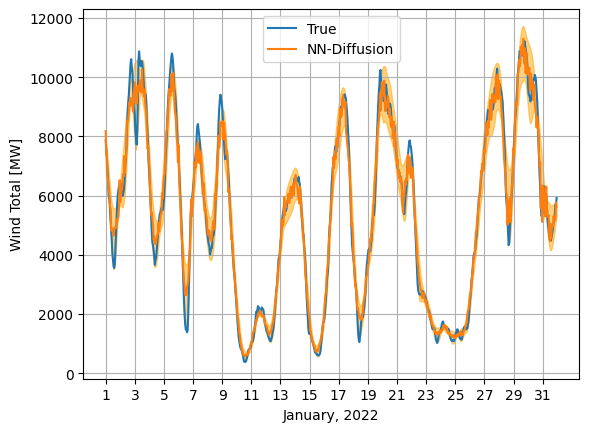
\includegraphics[width=1\linewidth]{wind-24-diff.png}
    \caption{}
    \label{fig:wind-24}
  \end{subfigure}
  \caption{(a) W-1 forecasts for January 2022 after the diffusion process. (b) W-24 forecasts }
  \label{fig:wind}
\end{figure}

\begin{figure}[t]
  \centering
  \begin{subfigure}{.45\textwidth}
    \centering
    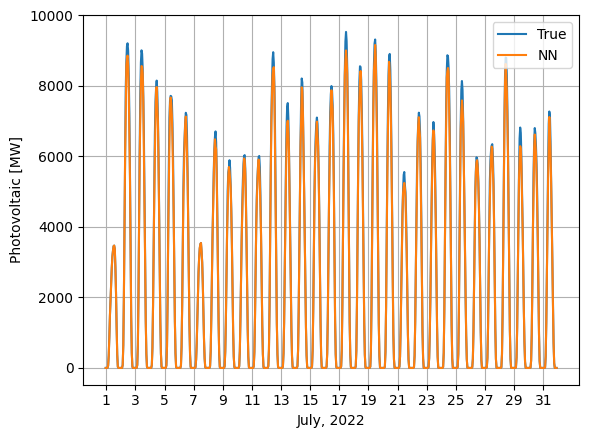
\includegraphics[width=1\linewidth]{solar-1.png}
    \caption{}
    \label{fig:solar-1}
  \end{subfigure}%
  \begin{subfigure}{.45\textwidth}
    \centering
    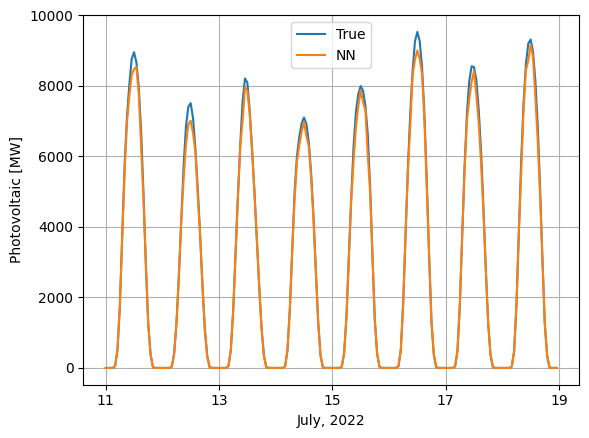
\includegraphics[width=1\linewidth]{solar-1-zoom.png}
    \caption{}
    \label{fig:solar-1-zoom}
  \end{subfigure}
  \begin{subfigure}{.45\textwidth}
    \centering
    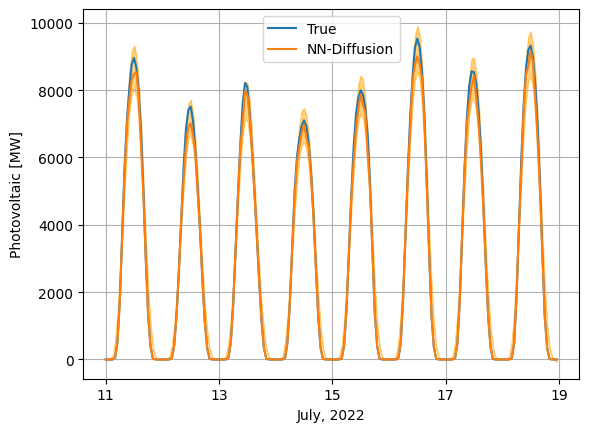
\includegraphics[width=1\linewidth]{solar-1-zoom-diff.png}
    \caption{}
    \label{fig:solar-1-zoom-diff}
  \end{subfigure}%
  \begin{subfigure}{.45\textwidth}
    \centering
    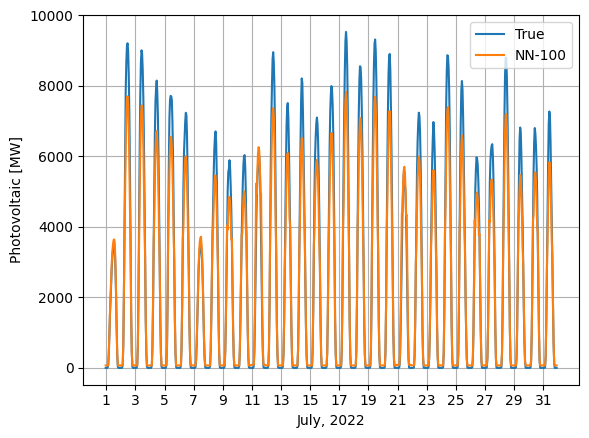
\includegraphics[width=1\linewidth]{solar-24.png}
    \caption{}
    \label{fig:solar-24}
  \end{subfigure}
  \caption{(a) S-1 forecasts for July 2022 by the prior conditioning model. (b) A lateral zoomed-in version of (a). (c) The forecasts after the diffusion process. Since the inference covers 100 different initial noise, they form a wide forecast distribution. (d) S-24 forecasts for July 2022.}
  \label{fig:solar}
\end{figure}

\section{Conclusion}

The diffusion process enhances predictions over the initial conditioning model. However, this method can be computationally intensive due to the numerous timesteps required, and it necessitates the optimization of additional hyperparameters, alongside nuisance parameters such as deciding which percentile to use and whether to include the original input data. The degree of improvement from diffusion models varies depending on the complexity or difficulty of the task, suggesting that these models may not always offer consistent benefits.

Another consideration is the role of probabilistic forecasts, which, while not always essential, can provide a valuable range of possible outputs. An open question remains whether an optimal prior conditioning model exists that could negate the need for diffusion, raising concerns about the potential limit of improvement achievable through this method. Moreover, the importance of noise, as observed in multiple distributions per sample, suggests that fine-tuning the initial noise could enhance predictions or reduce the computational burden of generating multiple predictions per sample. These aspects highlight the need for further research to fully exploit the benefits of diffusion models.


% Example citations: \cite{rolnick.2019}, \citet{rolnick.2019}, \citep{rolnick.2019}

% \subsection{Example Subsection}

% \begin{table}[h!]
%   \caption{Sample table title}
%   \label{sample-table}
%   \centering
%   \begin{tabular}{lll}
%     \toprule
%     \multicolumn{2}{c}{Part}                   \\
%     \cmidrule(r){1-2}
%     Name     & Description     & Size ($\mu$m) \\
%     \midrule
%     Dendrite & Input terminal  & $\sim$100     \\
%     Axon     & Output terminal & $\sim$10      \\
%     Soma     & Cell body       & up to $10^6$  \\
%     \bottomrule
%   \end{tabular}
% \end{table}

\printbibliography

\end{document}